%本章研究backorder对改进效果的影响

\chapter{Backorder对改进效果的影响}

在之前的讨论中,我们始终默认每一期的需求对后一期没有影响,也就是说未满足的订单将会被直接舍弃。实际上,作为供应商,如果不能按时交货,有时需要将订单记下,尽快补货,并且承受一定的惩罚。这种订单称为backorder。本章中,我们将讨论backorder对改进效果的影响。与前文不同的是,由于引入惩罚成本,本章中评价改进效果的指标不再是服务水平,而是考虑降低总成本。




\section{考虑Backorder成本的任意更新过程}

以汽车保险杠的生产线为例,为了使讨论简化,我们假设注塑环节需要的时间远大于喷涂环节,从而忽略喷涂环节的生产时间。也就是说,改进前后相比,单件产品的生产时间是不变的。

假设有N种颜色的成品,每种产品的需求都是独立到来的。每当需求到来时,如果该产品有库存,则立即满足该需求,且注塑机产生一个生产订单;如果没有库存,则产生一个backorder,并且在注塑机处产生一个生产订单。所有的生产订单采用先到先服务的策略。定义变量如下:

$s_i$:每种颜色初始库存;

$h$:库存成本率(成品与在制品相同);

$b$:backorder成本率(成品与在制品相同);

$D_i(t)$:直到$t$时刻,$i$产品的总需求;

$M_i(t)$:直到$t$时刻,$i$产品的总产量;

$I_i(t)$:$t$时刻的$i$产品库存,$I_i(t)=s_i+M_i(t)-\min\{s_i+M_i(t),D_i(t)\}$;

$B_i(t)$:$t$时刻的$i$产品backorder,$B_i(t)=D_i(t)-\min\{s_i+M_i(t),D_i(t)\}$;

$\phi_{i,N}(t)$:$t$时刻$i$产品的成本率,$\phi_{i,N}(t)=hI_i(t)+bB_i(t)$;

$\phi_N(t)$:$t$时刻所有产品的成本率,$\phi_N(t)=\sum_{i=1}^N\phi_{i,N}(t)$;

$\Phi_N(t)$:从初始时刻到$t$时刻的总成本,$\Phi_N(t)=\int_0^t\phi_N(u)\dif u$;

$s$:改进后的在制品初始库存;

$D(t)$:直到$t$时刻,改进后的在制品总需求;

$M(t)$:直到$t$时刻,改进后的在制品总产量;

$I(t)$:$t$时刻的在制品库存,$I(t)=s+M(t)-\min\{s+M(t),D(t)\}$;

$B(t)$:$t$时刻的在制品backorder,$B(t)=D(t)-\min\{s+M(t),D(t)\}$;

$\phi(t)$:$t$时刻在制品的成本率,$\phi(t)=hI(t)+bB(t)$;

$\Phi(t)$:改进后,从初始时刻到$t$时刻的总成本,$\Phi(t)=\int_0^t\phi(u)\dif u$。

接下来我们将证明,如果单纯把几种成品的库存合并为在制品库存,而不改变初始的库存总量,则改进后的总成本是低于改进前的总成本的。首先分析改进前后各变量之间的关系,显然有
\begin{equation}
s = \sum_{i=1}^N s_i,\qquad D(t) = \sum_{i=1}^N D_i(t),\qquad M(t) = \sum_{i=1}^N M_i(t)
\label{eq:改进前后的基本关系_backorder}
\end{equation}
根据以上关系可以推导出$\min\{s+M(t),D(t)\}\geq\sum_{i=1}^N\min\{s_i+M_i(t),D_i(t)\}$,过程如下:
\begin{align}
\min\{s+M(t),D(t)\} &= \min\left\{\sum_{i=1}^N s_i+\sum_{i=1}^N M_i(t),\sum_{i=1}^N D_i(t)\right\} \notag \\
&= \min\left\{\sum_{i=1}^N [s_i+M_i(t)],\sum_{i=1}^N D_i(t)\right\} \notag \\
&\geq \min\left\{\sum_{i=1}^N\min\{s_i+M_i(t),D_i(t)\},\sum_{i=1}^N\min\{s_i+M_i(t),D_i(t)\}\right\} \notag \\
&= \sum_{i=1}^N\min\{s_i+M_i(t),D_i(t)\}
\label{eq:局部放缩_backorder}
\end{align}
将不等式\ref{eq:局部放缩_backorder}代入$I(t)$的定义中,就能比较改进前后同一时刻的库存大小:
\begin{align}
I(t) &= s+M(t)-\min\{s+M(t),D(t)\} \notag \\
&\leq \sum_{i=1}^N s_i + \sum_{i=1}^N M_i(t) - \sum_{i=1}^N\min\{s_i+M_i(t),D_i(t)\} \notag \\
&= \sum_{i=1}^N [s_i+M_i(t)-\min\{s_i+M_i(t),D_i(t)\}] \notag \\
&= \sum_{i=1}^N I_i(t)
\label{eq:改进前后同一时刻库存比较_backorder}
\end{align}
同理可比较改进前后同一时刻backorder的大小:
\begin{align}
B(t) &= D(t)-\min\{s+M(t),D(t)\} \notag \\
&\leq \sum_{i=1}^N D_i(t) - \sum_{i=1}^N\min\{s_i+M_i(t),D_i(t)\} \notag \\
&= \sum_{i=1}^N [D_i(t)-\min\{s_i+M_i(t),D_i(t)\}] \notag \\
&= \sum_{i=1}^N B_i(t)
\label{eq:改进前后同一时刻backorder比较_backorder}
\end{align}
再将不等式\ref{eq:改进前后同一时刻库存比较_backorder}和\ref{eq:改进前后同一时刻backorder比较_backorder}代入$\phi(t)$的定义中,得到
\begin{equation}
\phi(t) = hI(t)+bB(t) \leq h\sum_{i=1}^N I_i(t) + b\sum_{i=1}^N B_i(t) = \phi_N(t)
\label{eq:改进前后成本率比较_backorder}
\end{equation}
公式\ref{eq:改进前后成本率比较_backorder}说明,改进后每时每刻的成本率都低于改进前同一时刻的成本率,自然地,改进后的总成本就低于改进前的总成本,即
\begin{equation}
\Phi(t)=\int_0^t\phi(u)\dif u \leq \int_0^t\phi_N(u)\dif u = \Phi_N(t)
\label{eq:改进前后成本比较_backorder}
\end{equation}
至此,已经证明了:如果单纯把几种成品的库存合并为在制品库存,而不改变初始的库存总量,则改进后的总成本低于改进前的总成本。

在这个系统中,需要企业决定的参数是初始库存。当需求分布和生产速率确定时,企业会选择一个最优的初始库存,使得成本最小。此处的成本是指长期运行的成本,所以这个最优的初始库存是由需求和生产在极限状态下的稳定分布决定的。Wolff(1989)\cite{wolff_stochastic_1989}证明:设$Q_i(t)=D_i(t)-M_i(t)$,且所有的到达都是独立同分布的更新过程,到达速率严格小于生产速率,则$Q_i(t)$是存在极限分布的。设此极限分布为$Q_i$。那么极限状态下的总成本率为
\begin{equation}
\psi_N(s_1,s_2,\ldots,s_N) = \sum_{i=1}^N\Big\{b[E(Q_i)-E(\min\{s_i,Q_i\})] + h[s_i - E(\min\{s_i,Q_i\})]\Big\}
\label{eq:极限总成本率_backorder}
\end{equation}
公式\ref{eq:极限总成本率_backorder}是初始库存$(s_1,s_2,\ldots,s_N)$的函数。对于每一个$b[E(Q_i)-E(\min\{s_i,Q_i\})] + h[s_i - E(\min\{s_i,Q_i\})]$,存在一个$s_i$使它取得最小值,我们将这个最优的$s_i$记为$s_i^*$。显然,使得总成本率$\psi_N(s_1,s_2,\ldots,s_N)$最小的一组$(s_1,s_2,\ldots,s_N)$是$(s_1^*1,s_2^*,\ldots,s_N^*)$。

同理,对于改进后的系统,设$Q(t)=D(t)-M(t)$,$Q(t)$的极限分布为$Q$。则改进后的极限状态下的成本率为
\begin{equation}
\psi(s) = b[E(Q)-E(\min\{s,Q\})] + h[s - E(\min\{s,Q\})]
\label{eq:改进后极限总成本率_backorder}
\end{equation}
同样存在一个$s$使$\psi(s)$取得最小值,将这个最优的$s$记为$s^*$。

显然,一般情况下,$s^*$和$\sum_{i=1}^Ns_i^*$是不相等的。也就是说,如果企业在改进前后都按照最优的库存策略来制定初始库存,那么改进前后的总库存不一定相等。这种情况下,改进后的总成本是否仍然低于改进前的总成本呢?利用之前的结论,我们仍然能够得到肯定的回答。

将我们要证明的结论转化为数学公式,目标就是证明$\psi(s^*)\leq\psi_N(s_1^*,s_2^*,\ldots,s_N^*)$。首先利用公式\ref{eq:改进前后成本比较_backorder}可以得到
\begin{equation}
\psi(\sum_{i=1}^Ns_i^*) \leq \psi_N(s_1^*,s_2^*,\ldots,s_N^*)
\label{eq:不等式右端_backorder}
\end{equation}
然后利用$s^*$的定义,由于$s^*$是使$\psi(s)$取得最小值的初始库存,所以$\psi(s^*)$小于等于任何$\psi(s)$值,其中包括$\psi(\sum_{i=1}^Ns_i^*)$。
\begin{equation}
\psi(s^*) \leq \psi(\sum_{i=1}^Ns_i^*)
\label{eq:不等式右端_backorder}
\end{equation}
由不等式\ref{eq:不等式右端_backorder}和\ref{eq:不等式右端_backorder}可得
\[
\psi(s^*) \leq \psi_N(s_1^*,s_2^*,\ldots,s_N^*)
\]
因此,即使在分别采取最优初始库存的情况下,改进后的成本率仍然比改进前要低。









\section{考虑Backorder成本的泊松过程}

上一节的定性结论适用于需求为任意更新过程的情况。如果要对改进前后的库存变化进行更量化的分析,需要知道需求的具体分布。在生产线的研究中,我们常常使用泊松过程作为需求和生产的分布。因此,现在我们假设需求和生产都是泊松过程。定义:

$\lambda_i$:$i$产品的到达速率;

$\lambda$:所有产品到达的总速率,$\lambda=\sum_{i=1}^N\lambda_i$;

$p_i$:$i$产品的需求占比,$p_i=\frac{\lambda_i}{\lambda}$;

$\mu$:生产速率;

$\rho$:需求产能比,$\rho = \frac{\lambda}{\mu}$,且$\rho<1$;

$D$、$M$、$Q$等变量定义与上一节相同。

根据Buzacott和Shanthikumar(1993)\cite{buzacott_stochastic_1993},$Q_i(t)$的极限分布是几何分布,记为$Q_i$,其概率分布为
\[
P(Q_i=n)=(1-r_i)r_i^n
\]
其中$r_i$的定义如下
\[
r_i = \frac{p_i\rho}{1-\rho+p_i\rho}
\]
由此可以计算出$I_i(t)$和$B_i(t)$各自的极限分布期望。分别记为$I_i$和$B_i$,则它们的期望为
\begin{align}
E(I_i) &= s_i - \frac{r_i(1-r_i^{s_i})}{1-r_i} \notag\\
E(B_i) &= \frac{r_i^{s_i+1}}{1-r_i} \notag 
\end{align}
然后得到极限成本率
\begin{equation}
\psi_N(s_1,s_2,\ldots,s_N) = E\left(\sum_{i=1}^N[hI_i+bB_i]\right)
\label{eq:极限成本率}
\end{equation}
公式\ref{eq:极限成本率}中,每一个$hI_i+bB_i$实际是是关于自变量$s_i$的函数,记为$C(s_i)$,则可以采用$C(s_i+1)-C(s_i)$的方式逐渐增大$s_i$,找到最优的$s_i^*$。根据Veatch和Wein(1996)\cite{veatch_scheduling_1996},这个最优值为
\begin{equation}
s_i^* = \left\lfloor\frac{\ln\gamma}{\ln r_i}\right\rfloor
\label{eq:泊松分布下的最优初始库存_backorder}
\end{equation}
其中$\gamma=\frac{h}{h+b}$。

公式\ref{eq:泊松分布下的最优初始库存_backorder}中为了符合实际需求而加入了取整符号。为了方便计算和推导,我们不对$s_i^*$向下取整,而是直接代入$\psi_N(s_1,s_2,\ldots,s_N)$,得到的是
\begin{equation}
\psi_N(s_1^*,s_2^*,\ldots,s_N^*) = h\sum_{i=1}^N\frac{\ln\gamma}{\ln\frac{p_i\rho}{1-\rho+p_i\rho}}
\label{eq:极限成本率最优值}
\end{equation}
同样的方法可以推出改进后的极限成本率为
\begin{equation}
\psi(s^*) = \frac{h\ln\gamma}{\ln\rho}
\label{eq:改进后极限成本率最优值}
\end{equation}

由公式\ref{eq:极限成本率最优值}和\ref{eq:改进后极限成本率最优值}可以比较改进前后的库存差,将这个差值记为$\Delta\psi$,则$\Delta\psi=\psi_N(s_1^*,s_2^*,\ldots,s_N^*)-\psi(s^*)$。

现在我们有了计算改进前后差值的公式,就可以进行一些数值实验。取$h=1$,$b=5$,$p_i=\frac{1}{N}$,计算$\Delta\psi$随产能比$\rho$的变化。数值实验的结果如图\ref{fig:改进前后极限成本率之差}所示。

\begin{figure}[htbp]
\centering
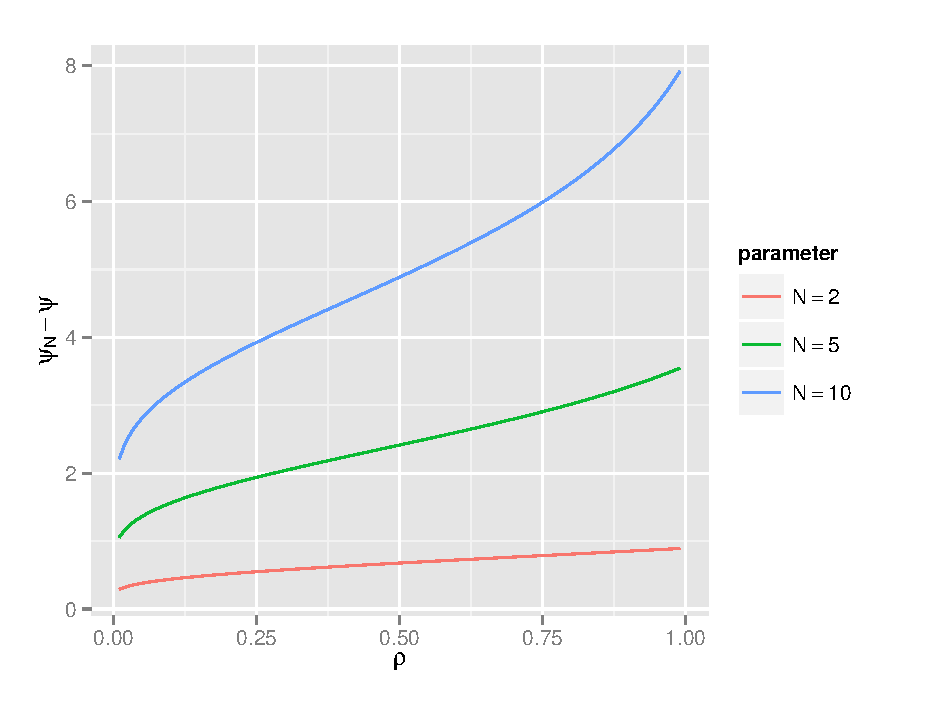
\includegraphics[width=15cm]{backorder_diff.eps}
\caption{改进前后极限成本率之差随$\rho$的变化}
\label{fig:改进前后极限成本率之差}
\end{figure}

毫无疑问,改进后的成本是小于改进前的成本的,这一点在前一节中已经得到定性的证明。除此之外,图\ref{fig:改进前后极限成本率之差}的三条曲线都显示,$\rho$越接近1,改进前后的库存之差越大。$\rho$代表的是需求产能比,$\rho = \frac{\lambda}{\mu}$。也就是说,需求量越接近产能,改进的效果越显著。这是与日常经验相符的,因为产能严重过剩的生产线一般不需要通过优化来挖掘潜力。

我们可以利用上述特性来估计改进效果的上限。求出$\rho \to 1$时,$\Delta\psi$的极限,就可以作为改进效果上限的一个估计。设所有需求的到达速率相同,都是$p_i=\frac{1}{N}$。则
\begin{equation}
\lim_{\rho\to 1}\Delta\psi = h\ln\gamma\lim_{\rho\to 1}\sum_{i=1}^N\left[\frac{1}{\ln\frac{p_i\rho}{1-\rho+p_i\rho}}-\frac{p_i}{\ln\rho}\right]
\label{eq:极限成本率差}
\end{equation}
对公式\ref{eq:极限成本率差}使用洛必达法则,可以得到
\begin{equation}
\lim_{\rho\to 1}\Delta\psi = \frac{1}{2}h(N-1)\ln\frac{h+b}{h}
\label{eq:极限成本率差结果}
\end{equation}

只要将具体的$h$、$b$、$N$的值代入公式\ref{eq:极限成本率差结果},就可以求出$\Delta\psi$在$\rho \to 1$时的极限值。该极限值可以作为对改进效果的上限的一种估计。企业可以通过这个简单的公式先估算可能获得的收益,再决定是否把其他因素考虑进来作更深的研究。





